\documentclass[12pt,a4paper]{article}
\usepackage{enumerate, amsmath, amsthm, multirow, mathrsfs, array, amssymb, indentfirst, latexsym, pstricks, graphicx, epstopdf, subfig, float, comment, bm, xpatch}
\usepackage{times}
\usepackage[labelfont=bf,textfont=bf]{caption}
\captionsetup[figure]{labelfont={bf},name={Fig.},labelsep=period}
\allowdisplaybreaks[1]
\newcommand{\halmos}{\rule{2mm}{2.5mm}}
\renewcommand{\qedsymbol}{\halmos}
\theoremstyle{plain}
\newtheorem{thm}{Theorem}[section]
\newtheorem{lem}[thm]{Lemma}
\newtheorem{cor}[thm]{Corollary}
\theoremstyle{definition}
\newtheorem{dfn}[thm]{Definition}
\newtheorem{exm}[thm]{Example}
\topmargin=-.6in
\textheight=9.6in
\oddsidemargin=5pt
\textwidth=38.5pc
\linespread{1.3}
\usepackage{hyperref}
\usepackage[round]{natbib}
\begin{document}

\begin{titlepage}

\thispagestyle{empty}
\begin{center}
\thispagestyle{empty}
\normalsize
\textsc{\textbf{SYNOPSIS OF}}\\
\bigskip

\Large{\textbf{EXPLOITING SPARSITY FOR DIRECTION OF ARRIVAL ESTIMATION ALGORITHMS IN LINEAR ARRAY}}\\

\bigskip \bigskip \bigskip \bigskip \bigskip \bigskip \bigskip \bigskip


\normalsize
\textbf{A THESIS}\\
\emph{to be submitted by}\\
\bigskip \bigskip \bigskip \bigskip
\normalsize
\textbf{ABHISHEK AICH}\\
\bigskip \bigskip \bigskip \bigskip
\emph{for the award of the degree}\\ \bigskip \bigskip
\emph{of}\\
\bigskip \bigskip
\normalsize
\textbf{MASTER OF SCIENCE (BY RESEARCH)}\\
\bigskip \bigskip \bigskip \bigskip \bigskip \bigskip \bigskip \bigskip
\centering

\includegraphics[width=32mm, height=32mm]{NITT.jpg}

\bigskip \bigskip
\normalsize
\textbf{DEPARTMENT OF ELECTRONICS AND COMMUNICATION ENGINEERING} \\
\normalsize
\textbf{
NATIONAL INSTITUTE OF TECHNOLOGY\\
TIRUCHIRAPPALLI -- 620 015}\\ \bigskip
\normalsize
\textbf{APRIL 2018}

\end{center}
\end{titlepage}
%end of cover page
\newpage
\section{INTRODUCTION}
Direction of arrival (DOA) estimation refers to the process of retrieving the direction information of several sources from the outputs of an number of receiving sensors that form a array. DOA estimation is a major problem in array signal processing and has wide applications in radar, sonar, wireless communications, etc. The study of DOA estimation methods has a long history. My algorithms like Capon’s beamformer were initially proposed for the estimation of closely spaced sources [\citet{R1}]. Since the 1970s, when Pisarenko found that the DOAs can be retrieved from data's second order statistics [\citet{R2}], a prominent class of methods designated as subspace-based methods have been developed, e.g., the multiple signal classification (MUSIC) and the estimation of parameters by rotational invariant techniques (ESPRIT) along with their variants [\citet{R3,R4,R5,R6,R7}].

Compressive sensing (CS) [\citet{R8,R9}] is being widely used in different research areas for its various properties. It utilizes the fact that the signals impinging on a sensor array are spatially sparse thus letting to exploit CS theory in DOA estimation problem. The novel contribution of CS-based DOA estimation methods is that very less time samples are required for high-resolution performance even in highly noisy environment. Recent works in DOA estimation have the introduction of CS to the framework. These new methods are motivated by techniques in sparse representation and compressed sensing methodology [\citet{R10,R11,R12}], and most of them have been proposed during the last decade. The sparse estimation (or optimization) methods can be applied in several demanding scenarios, including cases with no knowledge of the source number, limited number of time samples (even a single time sample), and highly or completely correlated sources. Due to these attractive properties they have been extensively studied and their popularity is reflected by the large number of publications.

It is important to note that there is a key difference between the common sparse representation framework and DOA estimation framework. To be specific, the studies of sparse representation have been focused on discrete linear systems. In contrast to this, the DOA parameters are continuous valued and the observed data are nonlinear in the angle domain. Depending on the model adopted, we can classify the sparse methods for DOA estimation into three categories, namely, on-grid, off-grid and gridless. For on-grid sparse methods, the data model is obtained by assuming that the true DOAs lie on a set of fixed grid points in order to straightforwardly apply the existing sparse representation techniques. While a grid is still required by off-grid sparse methods, the DOAs are not restricted to be on the grid. Finally, the recent gridless sparse methods do not need a grid, as their name suggests, and they operate directly in the continuous domain.

% Motivation
\section{MOTIVATION}
While DOA estimation is now a mature field with a solid theoretical basis and a large number of practical applications, it is still an evolving and quite active field of research. The major class of algorithms, the subspace based methods, suffer from certain well-known limitations. For example, they need a priori knowledge on the source number that may be difficult to obtain. Additionally, method's like Capon’s beamformer, MUSIC and ESPRIT are covariance-based and require a sufficient number of data snapshots to accurately estimate the data covariance matrix. Moreover, they can be sensitive to source correlations that tend to cause a rank deficiency in the sample data covariance matrix.

The main purpose of the DOA algorithm is to estimate the direction of incoming signals based on samples of received signals. The accuracy of estimation depends on the number of received signal samples. In general, DOA algorithms depend on two fundamental descriptions: steering vector and covariance matrix. Steering vector represents the response of the antenna array to a source in a certain direction. For multiple signals impinging an array, each signal direction will be associated with a unique steering vector. On top of that, the steering vector also describes the array geometry since different array configuration leads to unique expression. The covariance matrix involves the expectation of a received signal, but in practice this cannot be obtained; therefore, an average over a finite sample of received signals is normally used instead [\citet{R13}].

In many of the emerging applications, the traditional Nyquist rate of data acquisition is used but it is so high that we end up with far too many samples. It may simply be too costly, or even physically impossible, to build devices capable of acquiring samples at the required rate. Thus, despite tremendous advances in handling computational power, acquisition and processing of signals in areas such as medical imaging, remote surveillance, radar systems and data analysis continues to pose a tremendous challenge.

Compressive Sensing is a method of undersampling which aims at finding the most sparse representation of a signal that is able to achieve a target level with acceptable distortion. The CS beamformer proposed in [\citet{R14}] modifies the data model of the DOA estimation problem in terms of a CS problem and then solves it with traditional estimation based methods such as MVDR, MUSIC algorithms. This compensates for the price of the high complexity these algorithms need for the estimation of DOAs.

% Literature Survey 
\section{LITERATURE SURVEY}
One way to tackle the heavy computational complexity in subspace based algorithms is to introduce CS based Beamformer (CSB). Not only CSB reduces the data required, it also reduces the over flops required drastically [\citet{R14}]. 

CS sparse signal reconstruction algorithms can be broadly classified into two categories – Convex optimization based algorithms and the class of greedy algorithms. In this thesis, we mainly concentrate on a greedy algorithm called as orthogonal matching pursuit (OMP) [\citet{R15}]. The typical greedy sparse recovery approaches are basis pursuit (BP), compressive sampling matching pursuit (CoSaMP) [\citet{R16}], sparse Bayesian learning (SBL) and OMP [\citet{R17}]. Among these approaches, OMP is a compelling and favorable candidate for solving the DOA estimation problem due to its attractive properties. The main advantages of this algorithm are its low computational complexity and speed of recovery. Also, in addition to its fast implementation, OMP is also empirically advantageous in terms of recovery performance [\citet{R18}].

A literature survey reveals some of the most interesting applications of CS to DOA estimation problem in recent studies. Sparse recovery algorithms are equivalently effective with minimal snapshots, unlike as with multiple snapshots in case of conventional high-resolution DOA estimation algorithms. Hence, it is easier to work in scenarios like dynamic object tracking. The following work on application of CS to DOA estimation is a testimony to the advantages over traditional methods. In [\citet{R19}], author's have given an overview of these sparse methods for DOA estimation particularly recently developed gridless sparse methods. In [\citet{R20,R21}], a sparse covariance-based representation is exploited for source localization by applying a global matched filter. In [\citet{R22}], the $\ell_1$-SVD sparse recovery algorithm is proposed for DOA estimation. In [\citet{R23,R24}], an iterative re-weighted $\ell_1$ minimization is proposed for source estimation. In [\citet{R25}], a mixed $\ell_{2,0}$-norm based joint sparse approximation technique is proposed (JLZA-DOA) to solve the DOA estimation problem. Algorithms in [\citet{R26,R27,R28}] address the DOA estimation problem by directly representing the array output in time domain with an over-complete basis from the array response vector.
%

\section{OBJECTIVES AND SCOPE OF WORK}
\label{binfib}
This thesis focuses on utilizing an inherent property of Uniform Linear Array (ULA) based observed data, called sparsity. The main goal is to improve the complexity computations and the size of input data required to detect the directions of sources. The primary scope of this thesis is briefly summarized below:

\begin{itemize}
\item The first goal of this thesis is to derive stricter bounds for the dimensions of the measurement matrix employed in CSB-MUSIC algorithm.

\item The second goal of this thesis is to propose a novel and efficient CS beamformer root-MUSIC algorithm which follows the strict bounds introduced above. With this CSB introduction, the subspace deviation is analyzed and derived for this new algorithm in low snapshot scenario.

\item The third goal of this thesis is to overcome the inconsistency in power spectrum of OMP algorithm when employed for DOA estimation. In conjunction to this, a framework is to be designed for source distances estimation.

\end{itemize}
%\newpage
\section{SUMMARY OF THE RESEARCH WORK}

\subsection{Application of Compressive Sensing Based Beamformer to Music Algorithm for DOA Estimation}
%\setcounter{figure}{0}
\textbf{\emph{Background}}: The issue of reducing computational burden and its complexity while maintaining the adequate resolution has been a major problem in the area of DOA estimation. In recent works, it has been shown that by exploiting the sparsity of the observations obtained from the sensors, the computations can be greatly reduced without affecting resolution of the algorithm. This is done by introducing CSB to the picture. In this work, we proposed a new strict and improved bound to the dimensions of the measurement matrix to be used in the CSB-MUSIC algorithm which decrease the number of measurements still further. 

\subsubsection{CS Based Data Model}
Consider an ULA composed of \textit{N} omni-directional sensors. Let \textit{K} narrow-band signals impinge upon the ULA from distinct directions  \(\bm{\theta}=(\theta_1, \theta_2, \hdots, \theta_{\textit{K}}) \). Let \textit{L} be the number of time samples, \textit{d} and $\lambda$ be inter-element spacing and wavelength, respectively. It is assumed that sources are static, uncorrelated and the noise is independent from source, with zero-mean and variance $\sigma_n^2$. The ULA data model is given by
\begin{equation}\label{eq:a1}
\textbf{x}(t) = \textbf{A}(\textbf{$\theta$})\textbf{s}(t) + \textbf{w}(t);\quad \textit{t} = 1, 2, \hdots, \textit{L}
\end{equation}
where $\textbf{x}(t) \in \displaystyle\mathbb{C}^{\textit{N$\times$1}}$, $\textbf{A}(\textbf{$\theta$}) \in \displaystyle\mathbb{C}^{\textit{N$\times$K}}$, $\textbf{s}(t)\in \displaystyle\mathbb{C}^{\textit{K$\times$1}}$, $\textbf{w}(t)\in \displaystyle\mathbb{C}^{\textit{N$\times$ 1}}$.
\begin{figure}[h]
\centering
\includegraphics[width=90 mm]{figs/ULA_Poster.pdf}
\caption{DOA System Model}
\label{figa1}
\end{figure}
CS states that to reconstruct a \textit{s}-sparse signal \textbf{x}  $\in \displaystyle\mathbb{C}^{\textit{N$\times${1}}}$ (\(\textit{K} < \textit{N}\)) from  a measured signal \textbf{y}  $\in \displaystyle\mathbb{C}^{\textit{m$\times${1}}}$, only \(\textit{m} \geq \textit{s}\text{ln}\textit{N}\) number of measurements are needed. 
This is via the transformation
\begin{equation}\label{eq:a2}
\textbf{y} = \textbf{$\Phi$}\textbf{x}
\end{equation}
\noindent where $\Phi \in \displaystyle\mathbb{C}^{\textit{m$\times${N}}}$ is called the measurement matrix. From this, the CS based data model follows as (matrix form)
\begin{equation}\label{eq:a3}
\textbf{Y} = \Phi\textbf{A}\textbf{S} + \Phi\textbf{W}
\end{equation}
where \textbf{Y} = [\textbf{y}(1), \textbf{y}(2), $\hdots$, \textbf{y}(\textit{L})] $\in\mathbb{C}^{m\times L}$, \textbf{S} = [\textbf{s}(1), \textbf{s}(2), $\hdots$, \textbf{s}(L)] $\in\mathbb{C}^{K\times L}$ and \textbf{W} $\in\mathbb{C}^{N\times L}$ follows similarly as \textbf{Y}. In [\citet{R14}], it is shown that if the number of sources to locate is \textit{K}, the number of compressed measurements \textit{m} to be taken can be selected as 
\begin{equation}\label{eq:a4}
\textit{m} \geq \textit{K}\text{ln}\textit{N}
\end{equation}
But the CS beamformer is a modification applied to MUSIC algorithm, hence it doesn't use the generalized CS recovery methods to get the original signal or in this case, extract information from the signal. So when the bound was imposed as (\ref{eq:a4}), it was found that it could be still decreased without any compromise to the detection of DOAs.
\subsubsection{Proposed Bound to the Dimension of $\Phi$} 
We proposed the following lemma for a new strict bound of \textit{m} :
\begin{thm}
If the number of sources to locate is \textit{K} and the number of sensors is \textit{N} (\textit{N} $>$ \textit{K}), then the number of compressed measurements \textit{m} of the \textit{K}-sparse signal can be selected from the bound
\begin{align}\label{eq:a5}
  m &\in ( \textit{K}, \textit{N}]
\end{align}
\end{thm}  

\textbf{\emph{Results and discussion}}: 
An ULA is chosen with \textit{N} = 17 antenna elements. The number of signals is \textit{M} = 2 ( 0$^\circ$, 2$^\circ$). The number of
time snapshots is \textit{L} = 100. The compression matrix $\Phi$ has entries drawn from an identity matrix of size \textit{m}$\times$\textit{N}. The minimum \textit{m} by (\ref{eq:a4}) was found to be 6. But using our proposed lemma, the minimum \textit{m} = \textit{m}$_{new}$ was found to be 3 for which the DOAs were estimated. From the plot Fig. \ref{figa2} it can be observed that we were able to decrease m further by using our proposed lemma. This shows the superior optimality of our bound over the suggested one. 
\begin{figure}[h]
\centering
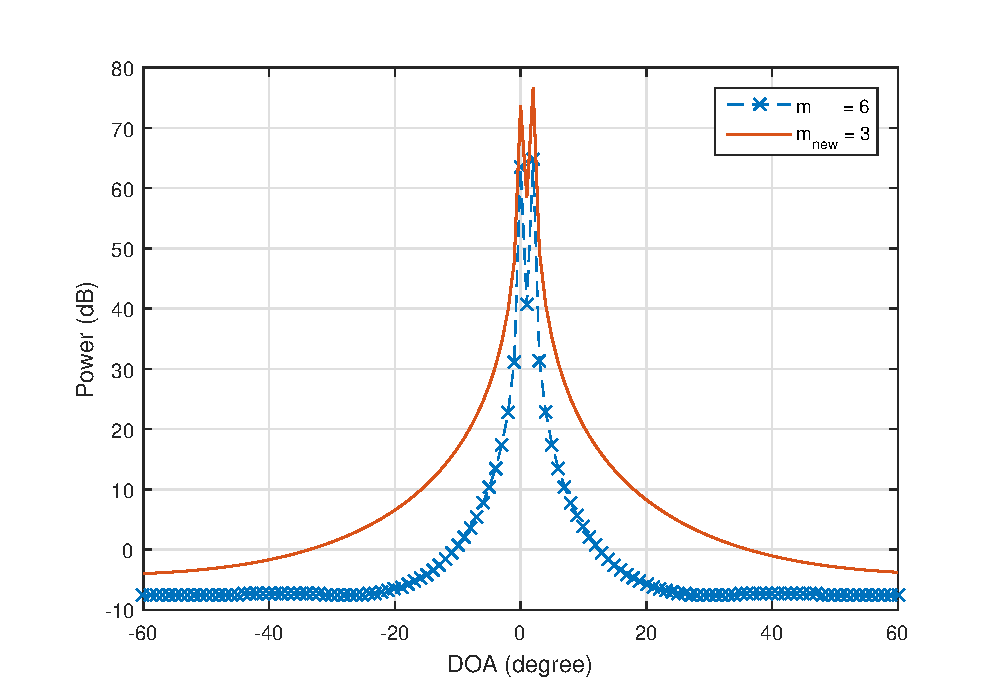
\includegraphics[width=90 mm]{figs/Spectrum_1.eps}
\caption{DOA Spectrum}
\label{figa2}
\end{figure}
\begin{figure}[h]
\centering
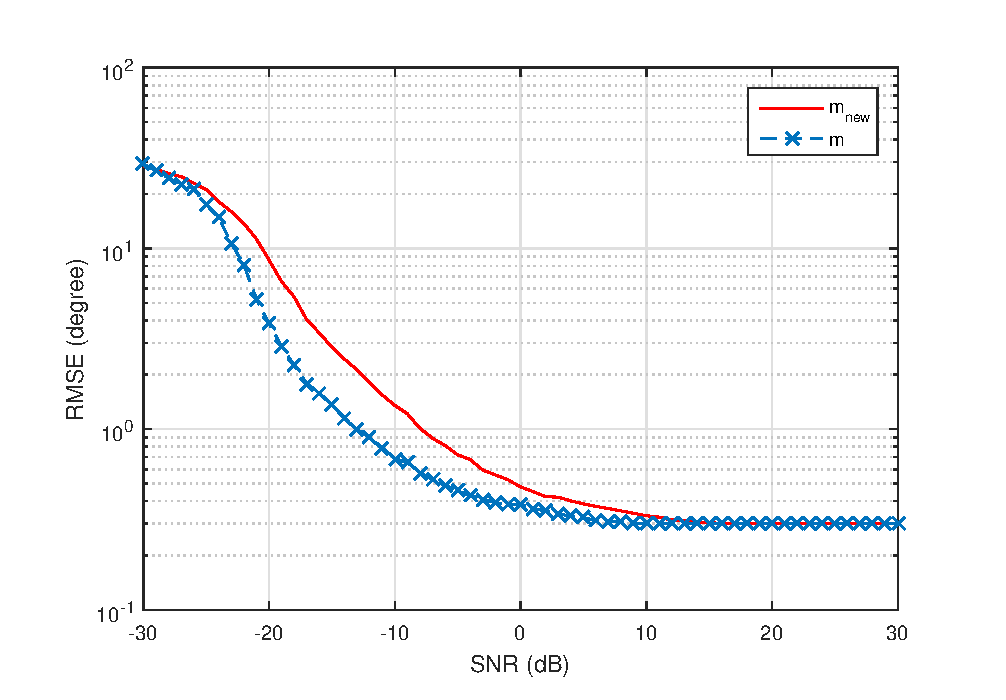
\includegraphics[width=90 mm]{figs/RMSE_2.eps}
\caption{RMSE \textit{vs} SNR analysis}
\label{figa3}
\end{figure}
\newline Again, an ULA chosen with \textit{N} = 30 antenna elements. The number of signals is \textit{K} = 1 ( 0$^\circ$). The number of time snapshots is \textit{L} = 100. The minimum m by (\ref{eq:a4}) was found to be 4. Using our proposed lemma, the minimum \textit{m} = \textit{m}$_{new}$ was found to be 2 and consecutively the DOA were estimated. Fig. \ref{figa3} shows the RMSE \textit{vs} SNR plot. It can be concluded that with little compromise in resolution for low SNR and no compromise in resolution for high SNR, our bound decreases the number of computations from $\mathcal{O}$(\textit{N}$^2$) to $\mathcal{O}$(\textit{m}$^2$).


\subsection{CSB - root - MUSIC Algorithm}
%\setcounter{figure}{0}
\textbf{\emph{Background}}: Subspace based techniques for direction
of arrival estimation need large amount of snapshots to detect source directions accurately. This poses a problem in the form of computational burden on practical applications. The introduction
of compressive sensing (CS) to solve this issue has become a norm in the last decade. In this work, a novel CS beamformer root-MUSIC algorithm is presented with a revised optimal measurement matrix
bound. With regards to this algorithm, the effect of signal subspace deviation under low snapshot scenario (e.g. target tracking) is analyzed.
\subsubsection{Proposed Algorithm}
Continuing from (\ref{eq:a3}), auto-correlation matrix of \textbf{Y} is given as
\begin{equation}\label{eq:a6}
\textbf{R}_{y} = \Phi\textbf{R}_{x}\Phi^{H}
\end{equation}
with $\textbf{R}_{x} = \mathbb{E}[\textbf{XX}^H]$
Though $\textbf{R}_{x} \in \displaystyle\mathbb{C}^{\textit{N$\times$N}}$, we have $\textbf{R}_{y} \in \displaystyle\mathbb{C}^{\textit{m$\times$m}}$ where \(m= K + 1\). 

The eigenvalue decomposition of $\textbf{R}_{y}$ is performed and after sorting in increasing order, first (\textit{m} - \textit{K}) eigenvectors, corresponding to first (\textit{m} - \textit{K}) eigenvalues, are arranged as columns of a matrix, say $\textbf{Q}_y \in \displaystyle\mathbb{C}^{\textit{K$\times$(m-K)}}$. $\textbf{Q}_y$ represents the noise subspace. Define \textit{z} $\triangleq \frac{{2}\pi{d}}{\lambda}$ sin($\theta$). Then, the steering vector given $\textbf{a}(\theta)$ is represented as
\begin{equation}\label{eq:a7}
\textbf{a}(z) = [1, z^{-1}, ..., z^{-(K-1)}] 
\end{equation}
Let \(\textbf{b}(z)=\Phi\textbf{a}(z)\). Then, according to [\citet{R7}], argument of the roots of the equation \begin{equation}
\textbf{b}^T(z^{-1})\textbf{Q}_y\textbf{Q}_y^H\textbf{b}(z)=0
\end{equation} 
gives the DOA estimates.
\subsubsection{Remarks on \textit{m} = \textit{K} + 1}
The bound \textit{m} of the measurement matrix was found to be sub-optimal, \textit{i.e.} it can further be decreased below the conventional CS theory. A strict bound on \textit{m} was hence, proposed given by the Theorem 5.1. Briefly, the theorem stated that the number of compressed measurements \textit{m} of the \textit{K}-sparse signal can be selected from the bound
\begin{flalign*}
  m &\in ( \textit{K}, \textit{N}]
\end{flalign*}
It can be directly concluded from the above theorem that the optimal value of \textit{m} for accurate detection of DOAs can be taken as \textit{K} + 1. This theorem also agrees for the root-MUSIC algorithm.
\subsubsection{Subspace Deviation in CS Beamformer}
With the introduction to CS beamformer to reduce the data requirement, it becomes a necessity to analyze the effect of low number of time samples on the performance of the proposed CS beamformer root-MUSIC algorithm. As we are using the CS-DOA model (\ref{eq:a3}) for the direction estimation, $\textbf{R}_{y}$ can be expanded as
\begin{align}
\widehat{\textbf{R}}_{y} = \textbf{B}\left\{\frac{1}{L}\sum_{t=1}^{L}\textbf{s}(t)\textbf{s}^H(t)\right\}\textbf{B}^H + \left\{\frac{1}{L}\sum_{t=1}^{L}\textbf{w}(t)\textbf{w}^H(t)\right\} \nonumber\\+ \underbrace{\textbf{B}\left\{\frac{1}{L}\sum_{t=1}^{L}\textbf{s}(t)\textbf{w}^H(t)\right\} + \left\{\frac{1}{L}\sum_{t=1}^{L}\textbf{w}(t)\textbf{s}^H(t)\right\}\textbf{B}^H}_\textbf{undesirable terms}
\end{align}
\noindent where $\widehat{\textbf{R}}_{y} = \frac{1}{L}\sum_{t=1}^L\textbf{y}(t)\textbf{y}^H(t)$ and $\textbf{B} = \Phi \textbf{A}$.
Define 
\begin{align*}
\textbf{Q} &\triangleq [\textbf{v}_{n(1)}, \textbf{v}_{n(2)}, \hdots, \textbf{v}_{n(m - K)}]\\
\textbf{P} &\triangleq [\textbf{v}_{s(1)}, \textbf{v}_{s(2)}, \hdots, \textbf{v}_{s(K)}]
\end{align*} 
where $\textbf{v}_{n(i)}$ ($\textit{i}^{th}$ column of \textbf{Q}) and $\textbf{v}_{s(j)}$ ($\textit{j}^{th}$ column of \textbf{P}) are the noise and signal eigenvectors respectively. In [\citet{R35}], the subspace deviation is defined as the average value of the energy of the estimated signal eigenvectors deviating to the true noise subspace. Mathematically, it is defined as
\begin{equation}\label{eq:a8}
\xi = \frac{1}{K}\sum_{j=1}^{K}\parallel\bm{\Gamma}_N\textbf{v}_{sj}\parallel_2^2
\end{equation}  
\noindent where \(\bm{\Gamma}_N \triangleq \textbf{Q}\textbf{Q}^H\). 
The expression in (\ref{eq:a8}), for the case of CS beamformer root-MUSIC algorithm gets simplified to 
\begin{equation}\label{eq:a9}
\xi = \frac{1}{K}\text{Tr}\{\textbf{V}^\dagger \triangle \textbf{R}_{y} \bm{\Gamma}_N \triangle \textbf{R}_{y} \textbf{V}^\dagger\}
\end{equation}  
\noindent where $\triangle \textbf{R}_{y}= \textbf{R}_{y} - \widehat{\textbf{R}}_{y}$, \(\textbf{R}_{y} =\mathbb{E}[\textbf{YY}^H]\) and $\textbf{V}^\dagger$ is the pseudo-inverse of $\textbf{V} = \textbf{R}_{y} - \sigma_n^2\textbf{I}_m$. Its expected value is given by 
\begin{equation}\label{eq:a10}
\mathbb{E}[\xi] = \frac{\sigma_n^2}{LK}\sum_{j=1}^{K}\frac{\lambda_{j+1}}{( \lambda_{j+1} - \sigma_n^2 )^2}
\end{equation}  

\noindent where $\lambda_j$ represents the eigenvalue of $\textbf{R}_{y}$.\\

\textbf{\emph{Results and discussion}}: 
For the DOA estimation spectrum, the SNR is kept as 15 dB. The ULA is chosen with \textit{N} = 7 sensors. Two non-coherent sources are considered with directions 20$^\circ$ , -50$^\circ$). The measurement matrix, $\Phi$ is chosen to be random Gaussian matrix with dimensions $\textit{m}\times \textit{N}$ where \textit{m} = 8. Fig. \ref{figa4} shows the plot for this simulation in which \textit{L} = 1000. 
\begin{figure}[h]
   \centering
    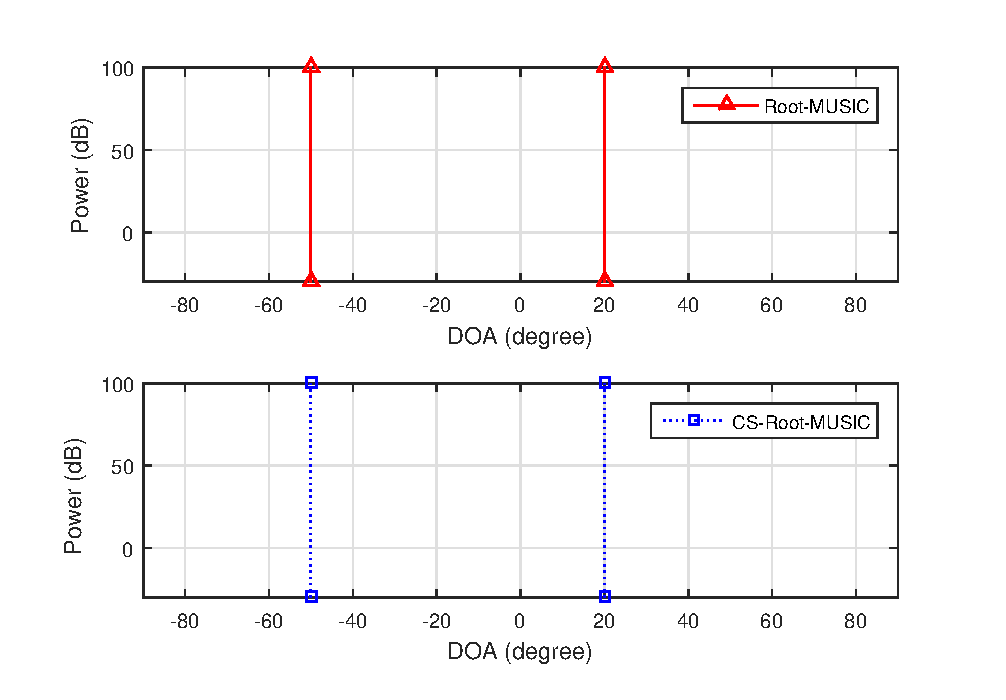
\includegraphics[height=7cm]{figs/DOA_Spectrum_1.eps}   
    \caption{DOA Spectrum}
    \label{figa4}
\end{figure}
\newline Next, the subspace deviation \textit{vs} SNR for different snapshots is evaluated with the theoretical approximation for root-MUSIC algorithm in comparison CS beamformer root-MUSIC algorithm with \textit{L} = 10. The ULA is chosen with \textit{N} = 10 sensors. The number of sources is \textit{K} = 2.
 \begin{figure}[H]
   \centering
    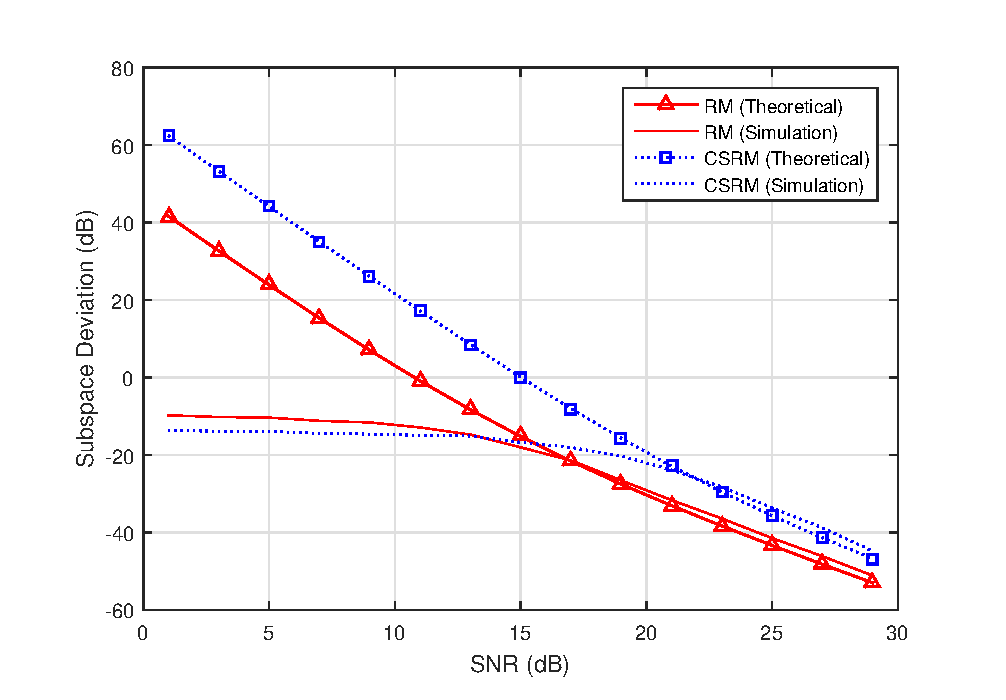
\includegraphics[height=7cm]{figs/SD_1.eps}
    \caption{Subspace deviation analysis (root-MUSIC (RM), CS beamformer root-MUSIC (CSRM))}
    \label{figa5}
\end{figure}

\subsection{Source Localization using Greedy Sparse Recovery Algorithms}
%\setcounter{figure}{0}
\textbf{\emph{Background}}:
We investigated the application of orthogonal matching pursuit (OMP) for DOA estimation for different scenarios, especially to tackle the case of coherent sources and observed inconsistencies in the results. In this work, a modified OMP algorithm was proposed to overcome these deficiencies by exploiting an orthogonality condition using only one time sample. This work is based on the probabilistic approach described in [\citet{R37,R38}]. The DOA estimation problem can be stated as a sparse recovery problem as follows:
\begin{align}\label{eq:4}
\tilde{\textbf{s}} = \min_{\tilde{\textbf{s}} \in \mathbb{C}^{L\times 1}} \Vert\tilde{\textbf{s}}\Vert_{0}\quad\text{s.t.}\quad\Vert\Phi\tilde{\textbf{A}}\tilde{\textbf{s}} - \textbf{y}\Vert_2^2 \le \epsilon
\end{align}
where $\epsilon >$ 0 is a measure of the noise level. Here $\Vert\tilde{\textbf{s}}\Vert_{0}$ is defined as the $\ell_0$ ``norm" (number of nonzero entries) of the \textit{M}-sparse vector $\tilde{\textbf{s}}\in\mathbb{C}^{M\times 1}$, $\tilde{\textbf{A}}$ is a dictionary matrix with columns as the steering vectors created for each scanned angle by the sensors. $\tilde{\textbf{A}}$ may be represented as
\begin{equation}
\tilde{\textbf{A}}(\theta)=
\begin{bmatrix}
1 & 1 & \cdots & 1\\
1 & e^{-j\rho_1} & \cdots & e^{-j\rho_{M - 1}}\\
\vdots & \vdots & \vdots \\
1 &  e^{-j(N - 1)\rho_1} & \cdots & e^{-j(N - 1)\rho_{M -1}} 
\end{bmatrix}
\end{equation}
Here \(\rho_q = \frac{{2}\pi{d}}{\lambda} sin(\theta_{q})\) with $\theta_q = 180^\circ\frac{q}{M}$, \textit{q} = $\frac{-(M-1)}{2}$, $\hdots$, 0, $\hdots$, $\frac{(M-1)}{2}$. It is important to note that the recovered signal vector $\tilde{\textbf{s}}$ will be of the following form
\[
    \tilde{s}_i= 
\begin{cases}
    s_{i} & \text{if}\quad \theta_{i} = \theta_1, \theta_2, \hdots, \theta_K\\
    0, & \text{otherwise}
\end{cases}
\] 
\noindent Clearly $\tilde{\textbf{A}}\in \mathbb{C}^{N\times M}$, $\tilde{\textbf{s}} \in\mathbb{C}^{M\times 1}$ with $\Phi\in \mathbb{C}^{m\times N}$.

\subsubsection{Inconsistency in OMP Algorithm}
We applied the OMP algorithm for DOA estimation for ULA data of only one time sample. In order to point out the discrepancies in the results, we did 10 Monte Carlo trials (Fig. \ref{figc1}) with 17 sensors, 3 sources ($\theta_1=0^{\circ}$, $\theta_2=40^{\circ}$ and $\theta_3=60^{\circ}$). 
\begin{figure}[h]
\centering
\includegraphics[height=7cm]{figs/Plot_7.pdf}
\caption{Plot for consistency of OMP Algorithm ( Monte Carlo trials = 10)}
\label{figc1}
\end{figure}

It can be observed that in trial 1, 4 and 6, only one source is detected. Similarly in trial 2, 3, 5 and 9, only two sources are detected whereas in trial 7, 8 and 10, all the three sources are detected. Clearly the results didn't detect all the DOAs in every simulation and hence the OMP algorithm is highly inconsistent and  unstable in performance.

\subsubsection{Proposed Direction Searching Function}
Now to resolve the above demonstrated problem, we move on to relax the RIP condition on the measurement matrix. This is done because intuitively we want to make this estimation of the support vector independent of the RIP condition. Also, it occurs in many sparse signal recovery problems, the condition of RIP is unnecessarily strict and that is not satisfied by many measurement matrices. Therefore, weaker versions of RIP are used and thus we use a \textit{weak}-1 RIP condition given below.
To bring in the effect of this weaker RIP condition, an orthogonality scheme is formulated which exploits the orthogonality of $\Psi\triangleq\Phi\tilde{\textbf{A}}$ and measured vector \textbf{y} which is independent of the RIP condition for detecting correct indices. This is implemented by using the following lemma obtained immediately from conventional beamforming.
\begin{lem} 
Let $\bm{\psi}_l$, $l\in [M]$ denote the \textit{l}$^{th}$ column of the augmented matrix $\Psi \triangleq \Phi\textup{$\tilde{\textbf{A}}$} \in \mathbb{C}^{m\times M}$. Assume that the entries of the measurement matrix $\Phi$ are i.i.d. zero-mean random variables. Then the objective function
\begin{equation}\label{eq:b1}
\textup{\textrm{U}}_\Gamma(\textbf{y}) \triangleq \mathbb{E}\vert\bm{\psi}^H_\Gamma\textup{\textbf{y}}\vert^2
\end{equation}
attains its maxima at $\Gamma\in$~\textup{supp[$\tilde{\textbf{s}}$]} in the absence of noise.
\end{lem}
Thus, we may expect the sample objective function 
\begin{equation}\label{eq:7i}
\textrm{T}_{\Gamma}(\textbf{y}) \triangleq \frac{\vert\textbf{y}^H\bm{\psi}_\Gamma\vert}{\Vert\bm{\psi}_\Gamma\Vert_2^2}
\end{equation}
to exhibit peaks at $\Gamma\in$~supp[$\tilde{\textbf{s}}$] for any particular realization of the random measurement matrix $\Phi$ as long as the SNR is not too low.

After recovering the partial support set of size \textit{r} in the above manner, the OMP algorithm will be called upon to act on the support reduced sparse signal vector to recover the remaining indices \textit{k} = \textit{p} - \textit{r} in supp[$\tilde{\textbf{s}}$].

\subsubsection{Proposed Framework for Source Distances Estimation}
We presented a method to estimate the distance of an source using the same sensor array. The set up geometry to estimate the distance of source is shown in  Fig. \ref{figc2}.
\begin{figure}[h]
\centering
\includegraphics[height=70mm]{figs/Linear_array_Distance.png}
\caption{Source distance estimation framework}
\label{figc2}
\end{figure}
Divide the received vector \textbf{x} $\in$ \( \mathbb{C} \)$^{\textit{N$\times$1}}$ in to two halves by the following method using a matrix \textbf{D} where     
\begin{align}\label{eq:11}
\textbf{D} = [\textbf{0}_{T \times (N - T)}, \textbf{I}_{T \times T}] 
\end{align} 
Then obtain $\textbf{x}_1$ as 
\begin{align}\label{eq:12}
\textbf{x}_1 = \textbf{D} \textbf{x} 
\end{align} 
with \[
    \textit{T}= 
\begin{cases}
    \frac{N}{2},& \textit{N}~\text{is even}\\
    \frac{N+1}{2},& \textit{N}~\text{is odd}
\end{cases}
\]  
The steps for finding the distance \textit{Z} are given as follows.
\begin{enumerate}[Step 1:~]
\item Find $\theta_1$ and $\theta_2$ using the proposed method by dividing the array frame as explained above.
\item Generate two straight-line equations
\begin{align}
\textit{x} &= \textit{m}_1 \textit{y}\label{eq:13}\\
\textit{x} &= \textit{m}_2 \textit{y} + \textit{C}\label{eq:14}
\end{align}
with \( \textit{m}_1 = \frac{\pi}{2} - \text{tan}~\theta_1\) ($\theta_1$ obtained from DOA estimation using Frame-1) and \( \textit{m}_2 = \frac{\pi}{2} - \text{tan}~\theta_2\) ($\theta_2$ obtained from DOA estimation using Frame-2). (\ref{eq:13}) is obtained from Frame-1 and (\ref{eq:14}) is obtained from Frame-2. Clearly \(\textit{C} = \textit{T}d\).
\item Solve the two straight line equations (\ref{eq:13}) and (\ref{eq:14}). The intersection of these two lines gives the position of the source. Denote this point as (a, b).Then distance \textit{Z} is calculated as
\begin{align}
\textit{Z} = \sqrt{\textit{a}^2 + \textit{b}^2}
\end{align}
\end{enumerate}

\begin{figure}[H] 
    \centering
    \includegraphics[height=7cm]{figs/Plot_9-eps-converted-to.pdf}
    \caption{Plot of Consistency of (a) OMP \textit{vs} (b) Proposed method}
    \label{figc3}
\end{figure}

\textbf{\emph{Results and discussion}}: 
We showed how the performance of the OMP algorithm is improved with our proposed algorithm. For this, we simulated a 3 source - 10 sensor setup in an environment of SNR = 10 db to show the consistency of both the algorithms (Fig. \ref{figc3}) for 10 Monte Carlo trials. The sources were selected as $\theta_1 = 60^\circ$, $\theta_2 = 40^\circ$ and $\theta_3 = 0^\circ$. It shows for all iterations, the proposed algorithm selects the true DOA correctly. For example, in the trial number 1 in (a), only $\theta_1$ is detected, in trial number 5, $\theta_2$ and $\theta_3$ are detected and in trial number 10, only $\theta_3$ is detected. In case of (b) \textit{i.e.} proposed algorithm, all sources $\theta_1$, $\theta_2$ and $\theta_3$ are detected in all trials from 1 - 10. This proves the claim that the proposed algorithm has overcome the deficiency of the OMP algorithm and is consistent in results.

%\newpage
\section{SUMMARY AND CONCLUSIONS}
In this thesis, sparse representation based system model is exploited for DOA estimation. In particular, the following works are done:

\begin{itemize}
\item CS-Beamformer based MUSIC algorithm was presented with improved strict bounds on the dimension of the measurement matrix. It was observed that the proposed modification to the algorithm showed a significant improvement in the computation complexity with negligible degradation in results.

\item A novel CS-Beamformer based root-MUSIC algorithms was proposed with improved strict bounds on the dimension of the measurement matrix. Further, its subspace deviation was analyzed in case of low snapshot scenario. 

\item The existing OMP algorithm was augmented with a novel objective function to overcome the inconsistencies in the power spectrum of DOAs in multiple Monte Carlo trials. A source distance calculation method was also proposed using the same array. 

\end{itemize}


\clearpage
\bibliographystyle{mystyle} 
\bibliography{references.bib}

\newpage
%\vspace{1cm}
\noindent \textbf{\normalsize 
\begin{center}
PROPOSED CONTENTS OF THE THESIS
\end{center}
} 
\vspace*{0.15cm}
\begin{description}
	\item[CHAPTER 1]  \textbf{INTRODUCTION}%\vspace{-0.75em}
	\begin{description}
     %\setlength\itemsep{-0.3em}
	\item[1.1] ULA System Data Model
	\item[1.2] Compressive Sensing
	\item[1.3] The Problem and Motivation
    \item[1.4] Contributions of the Work
    \item[1.5] Organization of the Thesis
\end{description}

	\item[CHAPTER 2] \textbf{LITERATURE REVIEW}%\vspace{-0.75em}
\begin{description}
%\setlength\itemsep{-0.3em}
	\item[2.1] Subspace Based DOA Estimation Algorithms  
	\item[2.2] Compressive Sensing Based Sparse Recovery Algorithms  
	\item[2.3] Sparse Framework Based DOA Estimation Algorithms
   \end{description}
   
\item[CHAPTER 3] \textbf{COMPRESSIVE SENSING BASED MUSIC ALGORITHM}%\vspace{-0.75em}	
\begin{description}
%\setlength\itemsep{-0.3em}
    \item[3.1] Introduction
    \item[3.2] Preliminaries
    \item[3.3] CS Beamformer MUSIC Algorithm %\vspace{-0.5em}
		\begin{description}
		\item[3.3.1] Choosing a Proper Measurement Matrix $\Phi$
        \item[3.3.2] Proposed Bound to the Dimension of $\Phi$
		\end{description}
	\item[3.4] Results and Discussion
\end{description}

\item[CHAPTER 4]\textbf{COMPRESSIVE SENSING BASED ROOT - MUSIC ALGORITHM}%\vspace{-0.75em}
\begin{description}%\setlength\itemsep{-0.3em}
	\item[4.1] Introduction
	\item[4.2] Proposed Algorithm %\vspace{-0.5em}
		\begin{description}
		\item[4.2.1] CS beamformer root-MUSIC Algorithm
        \item[4.2.2] Remarks on \textit{m} = \textit{K} + 1
		\end{description}
	\item[4.3] Subspace Deviation in CS Beamformer %\vspace{-0.5em}
    \item[4.4] Results and Discussion\\*\\
\end{description}

\item[CHAPTER 5]  \textbf{OVERCOMING DOA SPECTRUM INCONSISTENCY OF ORTHOGONAL MATCHING PURSUIT ALGORITHM}%\vspace{-0.75em} 
\begin{description}%\setlength\itemsep{-0.3em}
  \item[5.1] Introduction
  \item[5.2] Preliminaries
  		\begin{description}
		\item[5.2.1] CS Data Model for DOA Estimation
        \item[5.2.2] Application of OMP Algorithm
		\end{description}
  \item[5.3] Proposed Algorithm %\vspace{-0.5em}
		\begin{description}
		\item[5.3.1] On the Bound of Weak-1 RIP Constant
        \item[5.3.2] Distance of Sources
		\end{description}
  \item[5.4] Results and Discussion
\end{description}

\item[CHAPTER 6] \textbf{SUMMARY AND CONCLUSION}%\vspace{-0.75em}
\begin{description}%\setlength\itemsep{-0.3em}
	\item[6.1] Summary and Conclusion
	\item[6.2] Future Work
\end{description}

\end{description}
\newpage
\begin{center}
\textbf{THE THESIS IS BASED ON THE FOLLOWING PUBLICATIONS}
\end{center}
\bigskip

\begin{itemize}

\item[I] \textbf{PRESENTATIONS IN CONFERENCES}

\begin{enumerate}[ 1. ]
\item \textbf{Aich, A.} and \textbf{P. Palanisamy} (2016) A strict bound for dimension of measurement matrix for CS beamformer MUSIC algorithm. \emph{IEEE Region 10 Conference (TENCON-2016)}, NTU Singapore, 2602-2605.

\item \textbf{Aich, A.} and \textbf{P. Palanisamy} (2017) A novel CS beamformer root-MUSIC algorithm and its subspace deviation analysis. \emph{IEEE Region 10 Conference (IEEE TENCON-2017)}, Penang, Malaysia, 1404-1408.

\item \textbf{Aich, A.} and \textbf{P. Palanisamy} (2017) On application of OMP and CoSaMP algorithms for DOA estimation problem. \emph{IEEE International Conference on Communication and Signal Processing (IEEE ICCSP-2017)}, Chennai, India, 1983-1987.

\item \textbf{Aich, A.} and \textbf{P. Palanisamy} (2017) On-grid DOA estimation method using Orthogonal Matching Pursuit. \emph{IEEE International Conference on Signal Processing and Communication (IEEE ICSPC-2017)}, Coimbatore, India, 483-487.
\end{enumerate}

\item[II] \textbf{REFERRED JOURNALS}
\begin{enumerate}[ 1. ]
\item \textbf{Aich, A., P. Palanisamy,} and \textbf{N. Kalyanasundaram} A Novel Sparse recovery based DOA estimation algorithm by relaxing the RIP constraint. \emph{IET-Signal Processing (Revision submitted)}.

\end{enumerate}
\end{itemize}

 \end{document}